\let\negmedspace\undefined
\let\negthickspace\undefined
%\RequirePackage{amsmath}
\documentclass[journal,12pt,twocolumn]{IEEEtran}
 \usepackage[utf8]{inputenc}
 \usepackage{graphicx}
 \usepackage{amsmath}
 \usepackage{amsfonts}
 \usepackage{amssymb}
 \usepackage{enumitem}
\usepackage{mathtools}
\usepackage[breaklinks=false]{hyperref}
\usepackage{listings}
\usepackage{calc}

\newcommand{\BEQA}{\begin{eqnarray}}
\newcommand{\EEQA}{\end{eqnarray}}
\newcommand{\define}{\stackrel{\triangle}{=}}
\bibliographystyle{IEEEtran}
%\bibliographystyle{ieeetr}

\let\vec\mathbf

\providecommand{\abs}[1]{\left\vert#1\right\vert}
\providecommand{\res}[1]{\Res\displaylimits_{#1}}
\providecommand{\norm}[1]{\left\lVert#1\right\rVert}
\providecommand{\brak}[1]{\ensuremath{\left(#1\right)}}
\newcommand{\myvec}[1]{\ensuremath{\begin{pmatrix}#1\end{pmatrix}}}
\newcommand{\mydet}[1]{\ensuremath{\begin{vmatrix}#1\end{vmatrix}}}
\newcommand{\question}{\noindent \textbf{Question: }}
\newcommand{\solution}{\noindent \textbf{Solution: }}


\title{Assignment 1}
\author{Vishal Vijay Devadiga (CS21BTECH11061)}
\date{}
\begin{document}
% make the title area
\maketitle
\question
\begin{enumerate}[label=]
\item A(-1, 3), B(4,2) and C(3,-2) are the vertices of a triangle.
\begin{enumerate}
    \item Find the coordinates of the centroid G of the triangle
    \item Find the equation of the line through G and parallel to AC.
\end{enumerate}
\end{enumerate}
\solution
\begin{enumerate}
	\begin{figure}[h]
	\centering
	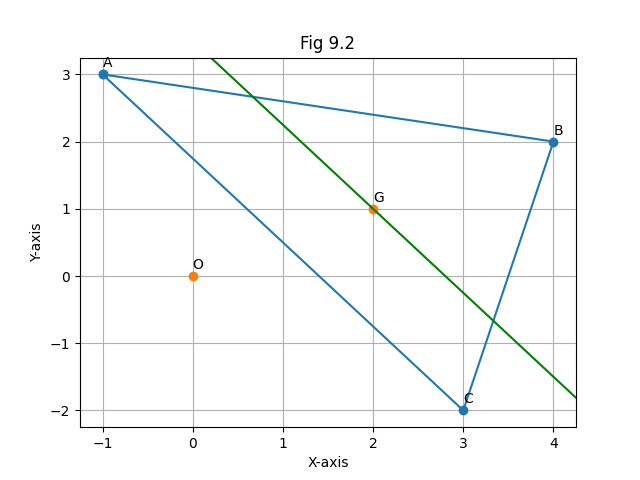
\includegraphics[width=\columnwidth]{./figs/9.2.png}
	\end{figure}
\item Let $\vec{A}, \vec{B}, \vec{C}$ be the points vectors.
	\begin{align}
		\vec{A} = \myvec{-1 \\ 3} ,
		\vec{B} = \myvec{4 \\ 2}  ,
		\vec{C} = \myvec{3 \\ -2}
	\end{align}
	Using centroid formula,the desired point vector $\vec{G}$ is given by:
    \begin{align}
        \vec{G}&= \frac{1}{3}\brak{\vec{A} + \vec{B} + \vec{C}}
        \\
        &= \frac{1}{3}\brak{\myvec{-1 \\ 3} + \myvec{4 \\ 2} + \myvec{3 \\ -2}}
        \\
        &=\frac{1}{3}\myvec{6 \\ 3}
        \\
        &= \myvec{2 \\ 1}
    \end{align}
    $\vec{G}$ is the point vector $\myvec{2 \\ 1}$
\item Let L be the line that passes through $\vec{G}$ such that $L \parallel AC$
    The direction vector of $AC$, $\vec{m}$, is given by,
    \begin{align}
    \vec{m} &= \vec{A} - \vec{C}
    \\
	&= \myvec{-1 \\ 3} - \myvec{3 \\ -2}
	\\
	&= \myvec{-4 \\ 5}
    \end{align}
    Normal vector of the line is $\vec{n}$, such that
    \begin{align}
	&\vec{m}^{\top}\vec{n} = 0
	\\
	\implies &\myvec{-4 & 5}\vec{n} = 0
	\\
	\implies &\vec{n} = \myvec{5 \\ 4}
	\\
	\implies &\vec{n}^{\top} = \myvec{5 & 4}
    \end{align}
    The normal equation of the line L is given by, 
    \begin{align}
	&\vec{n}^{\top}\brak{\vec{x} - \vec{G}} = 0
	\\
	\implies &\myvec{5 & 4}\brak{\vec{x} - \myvec{2 \\ 1}} = 0
	\\
	\implies &\myvec{5 & 4}\vec{x} - \myvec{5 & 4}\myvec{2 \\ 1} = 0
	\\
	\implies &\myvec{5 & 4}\vec{x} = 14
    \end{align}
    Thus, line L $\equiv \myvec{5 & 4}\vec{x} = 14$
\end{enumerate}
\end{document} 
